\documentclass[15pt]{standalone}
\usepackage{xcolor}
\usepackage{tikz}
\usepackage{pgfplots}
\definecolor{slide}{HTML}{d5002d}
\definecolor{original}{HTML}{005aff}
\definecolor{scaled}{HTML}{03af7a}
\begin{document}
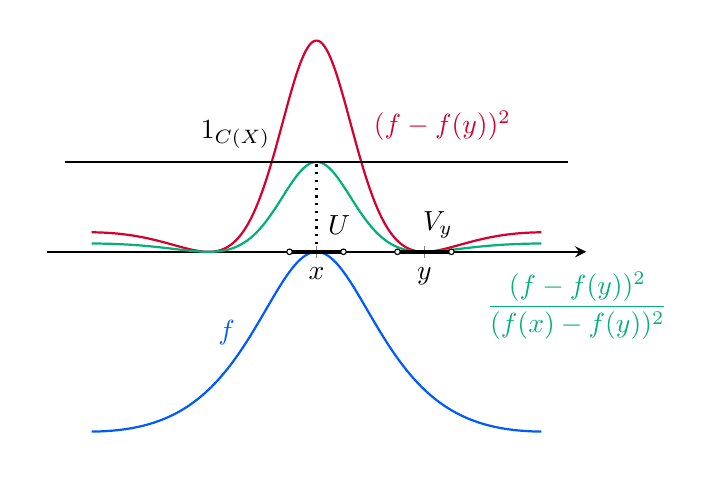
\begin{tikzpicture}
    \begin{axis}[
        axis equal,
        axis x line=middle,
        axis line style=thick,
        xmin=-3,
        xmax=3,
        ymin=-1.8,
        ymax=1.8,
        xtick={0, 1.2},
        xticklabels={$x$, $y$},
        x tick style={draw},
        x axis line style={draw},
        ytick={},
        yticklabels={},
        y axis line style={draw=none},
        y tick style={draw=none},
        samples=300,
        clip=false
    ]
    \def\SCALE{1.8};
    \def\SIGMA{0.3};
    \def\A{-2.5};
    \def\B{2.5};
    \def\yy{1.2};
    \addplot[color=original, thick][domain=\A:\B] {\SCALE * cos(deg(x))/(x^2 + 1) - \SCALE};
    \addplot[color=slide, thick][domain=\A:\B] {(\SCALE * cos(deg(x))/(x^2 + 1) - \SCALE * cos(deg(\yy))/(\yy^2 + 1) )^2};
    \addplot[color=scaled, thick][domain=\A:\B] {(\SCALE * cos(deg(x))/(x^2 + 1) - \SCALE * cos(deg(\yy))/(\yy^2 + 1) )^2 / (\SCALE * cos(deg(0)) - \SCALE * cos(deg(\yy))/(\yy^2 + 1) )^2};
    \node[color=original] (original) at (axis cs:-1, -0.9) {$f$};
    \node[color=slide] (slide) at (axis cs:1.4, 1.4) {$(f - f(y))^2$};
    \node[color=scaled] (scaled) at (axis cs:2.9, -0.6) {$\displaystyle \frac{(f - f(y))^2}{(f(x) - f(y))^2}$};

    \draw[fill=white, opacity=1] (axis cs:-0.3, 0) circle[radius=1pt];
    \draw[fill=white, opacity=1] (axis cs:0.3, 0) circle[radius=1pt] {};
    \draw[ultra thick] (axis cs: -0.275, 0) -- (axis cs: 0.275, 0);
    \node at (axis cs: 0.25, 0.3) {$U$};
    \draw[fill=white, opacity=1] (axis cs:0.9, 0) circle[radius=1pt];
    \draw[fill=white, opacity=1] (axis cs:1.5, 0) circle[radius=1pt] {};
    \draw[ultra thick] (axis cs: 0.925, 0) -- (axis cs: 1.475, 0);
    \node at (axis cs: 1.35, 0.3) {$V_y$};

    \draw[thick] (axis cs:-2.8, 1) -- (axis cs:2.8, 1);
    \draw[thick, dotted] (axis cs: 0, 0) -- (axis cs: 0, 1);
    \node[] (line1) at (axis cs:-0.9, 1.3) {$1_{C(X)}$};

    \end{axis}
    \end{tikzpicture}
\end{document}
